\chapter{Comparison of Methods}
\label{chap:Testing}

\vspace{-1cm}

This chapter compares the performance of various methods used in the UAV navigation system, focusing on accuracy, runtime, and robustness. The evaluation includes feature detectors, local feature matchers, rotational and translational estimators, and optimization techniques. Each method is tested across multiple datasets to assess generalization and suitability for real-world UAV applications.


\vspace{-0.5cm}
\section{Testing Setup}
\vspace{-0.25cm}


This section outlines the framework used to evaluate the performance of the proposed UAV navigation methods. The evaluation focuses on three primary metrics: accuracy, runtime, and robustness. These metrics are critical to ensure that the navigation system can reliably operate under diverse and challenging conditions, reflecting real-world scenarios where the UAV may encounter varying environmental factors.

Note that understanding the testing setup is important for interpreting the subsequent results section.

\subsection{Critical Testing Pipeline Understanding}

The aim of these tests is to compare different methods, rather than to evaluate the overall system performance. The tests were conducted under intermediary development pipeline methods that are not listed, and not under optimized runtime or accuracy settings for the entire system; however, when testing methods within a particular stage, all other stages and parameters were held constant to ensure fair comparisons. Additionally, non-testing parameters and methods were set to optimal or near-optimal values to ensure that each method was evaluated under favorable conditions. This choice ensures that comparisons were still fair without having to iteratively retest as improvements were made. Therefore, the results presented are not indicative of the overall system performance, and no conclusions about the system's overall performance should be drawn from this chapter.

\subsection{Datasets}

Five distinct datasets were created to rigorously evaluate the methods' generalization and performance across diverse environments. These datasets were captured using Google Earth and involved both translational and rotational movements, simulating typical UAV navigation tasks. Although the primary transformations were translation and rotation, there were subtle perspective and scale distortions introduced by the 3D rendering in Google Earth. The magnitude of these distortions is implicitly addressed by the degrees of freedom of the transformation estimation methods used, negating the need to quantify these distortions explicitly.

To maximize the utility of the datasets, the same images are used for both the GNSS-available and GNSS-denied stages. During the GNSS-available stage, all 15 images are streamed and stored along with their features and telemetry data. The first 5 images are used to infer the fixed pixel-to-meter factor, which is related to the camera focal length and UAV altitude. Subsequently, during the GNSS-denied stage, the 15 images have their location and heading estimated without GNSS data. Importantly, each image in the GNSS-denied stage recomputes its features and does not rely on any ground truth telemetry or use itself as a reference image, ensuring a fair test. Additionally, the images are spaced sufficiently to introduce challenges in the datasets.

The datasets have various properties to ensure that the tests are challenging yet feasible, and to mimic real-world data. The datasets were captured at altitudes corresponding to ground heights of 5–7 km, using images with a resolution of 1920×972 pixels. The specific resolution was chosen to eliminate image text that could cause false positive matches. The radial movement between frames varies between 300 and 700 pixels, depending on the image and the best match found. This corresponds to around 50\% to 80\% overlap between frames. Although the accuracy of the distance in metres is dependent on the translation size between frames, the method that yields the lowest meter error also produces the lowest overall error. Therefore, this variability does not impact the comparison of methods based on meter measurements. Each dataset consists of 15 images, balancing testing time with sufficient evaluation of the methods' performance.

The datasets used in this analysis encompass a range of terrains and motion types. The CITY1 and CITY2 datasets were captured in Cape Town, with CITY1 incorporating both rotational and translational changes between frames, whereas CITY2 focuses solely on translational movements and is taken at a significantly lower altitude, as per Table~\ref{tab:tilted_camera}. The ROCKY dataset, collected in the semi-arid Karoo region, features rugged terrain with sparse vegetation and includes both translations and rotations. The DESERT and AMAZON datasets, captured in the Sahara Desert and Amazon Rainforest respectively, are marked by sparse, repetitive patterns that pose challenges for feature extraction and matching. These datasets involve both translations and rotations and are difficult even for human observers to distinguish frame-to-frame differences.



Examples of the datasets are shown below:

\begin{figure}[H]
    \centering
    \begin{minipage}{0.4\textwidth}
        \centering
        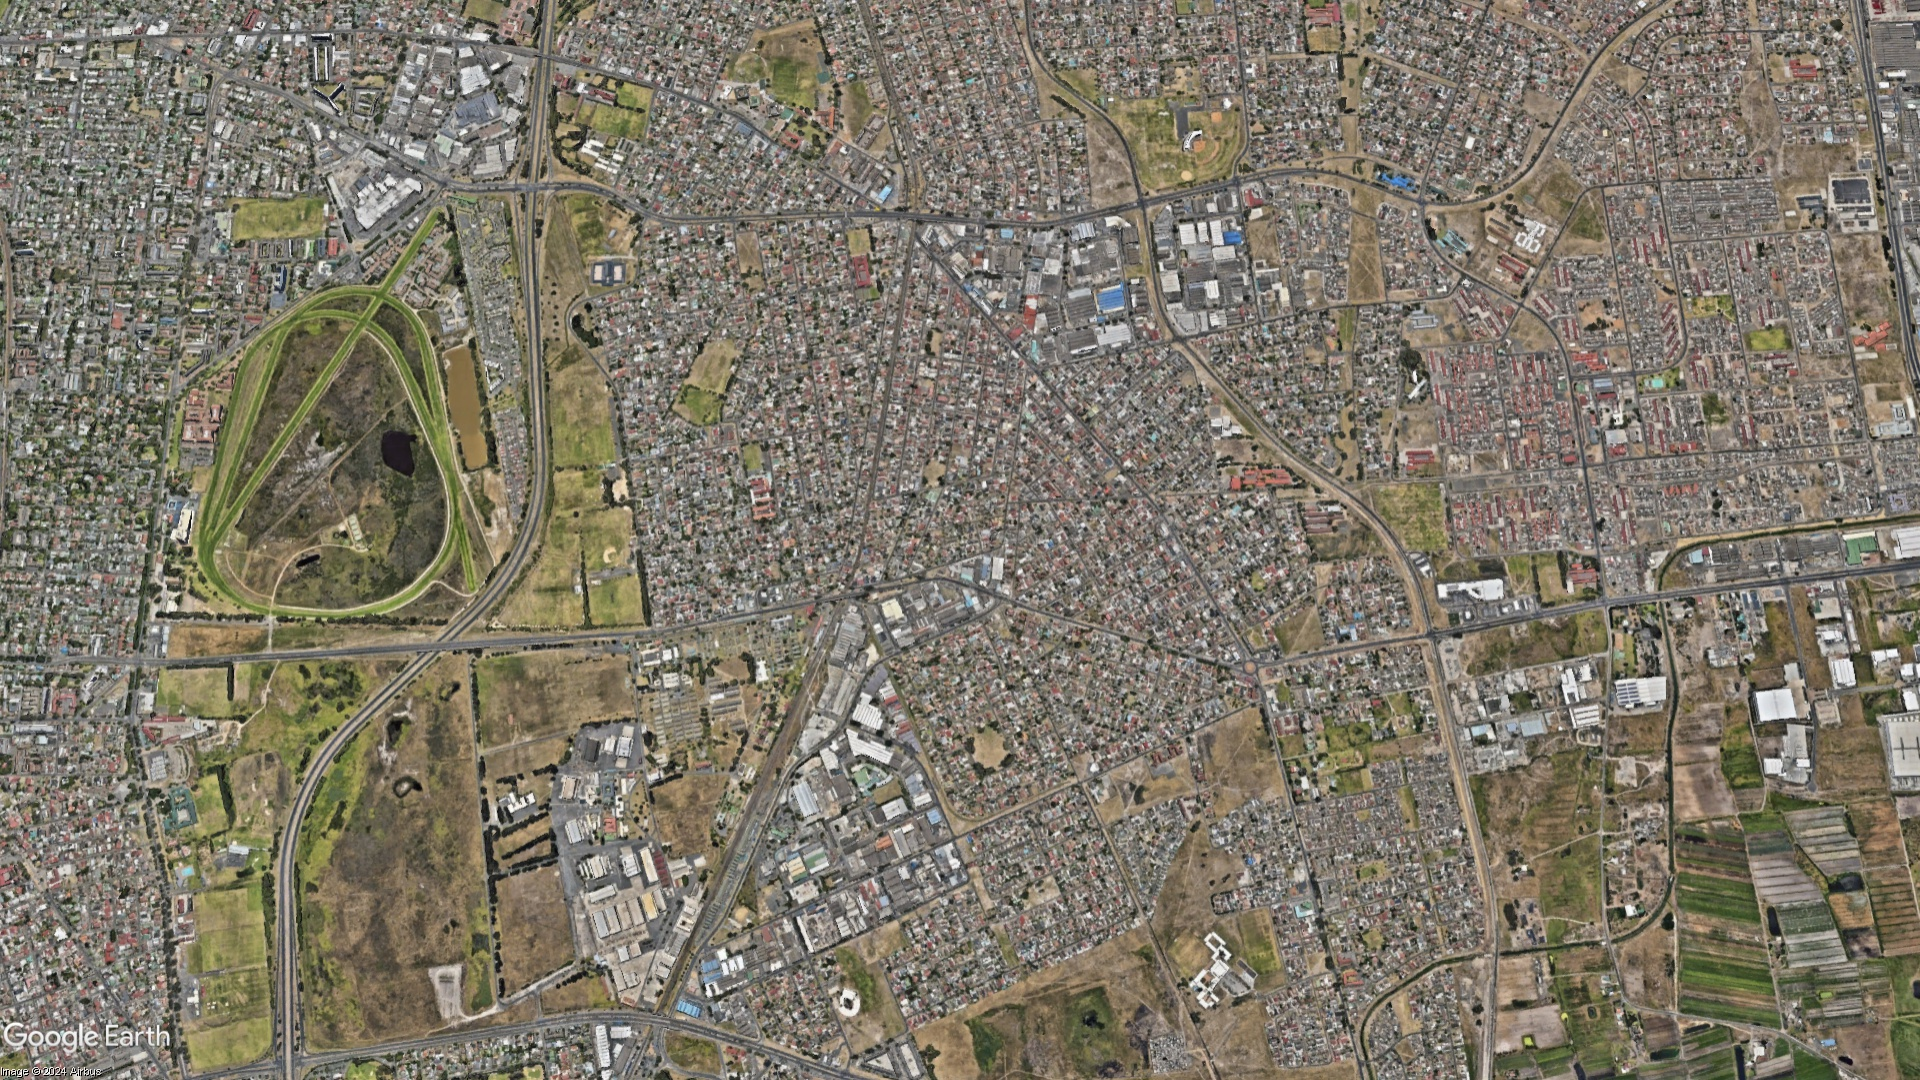
\includegraphics[width=\textwidth]{./Chapter 4/DEMODATASETS/CITY1.jpg}
        \caption{Examples of the CITY1 and CITY2 Datasets.}
        \label{fig:CITY12}
    \end{minipage}\hfill
    \begin{minipage}{0.4\textwidth}
        \centering
        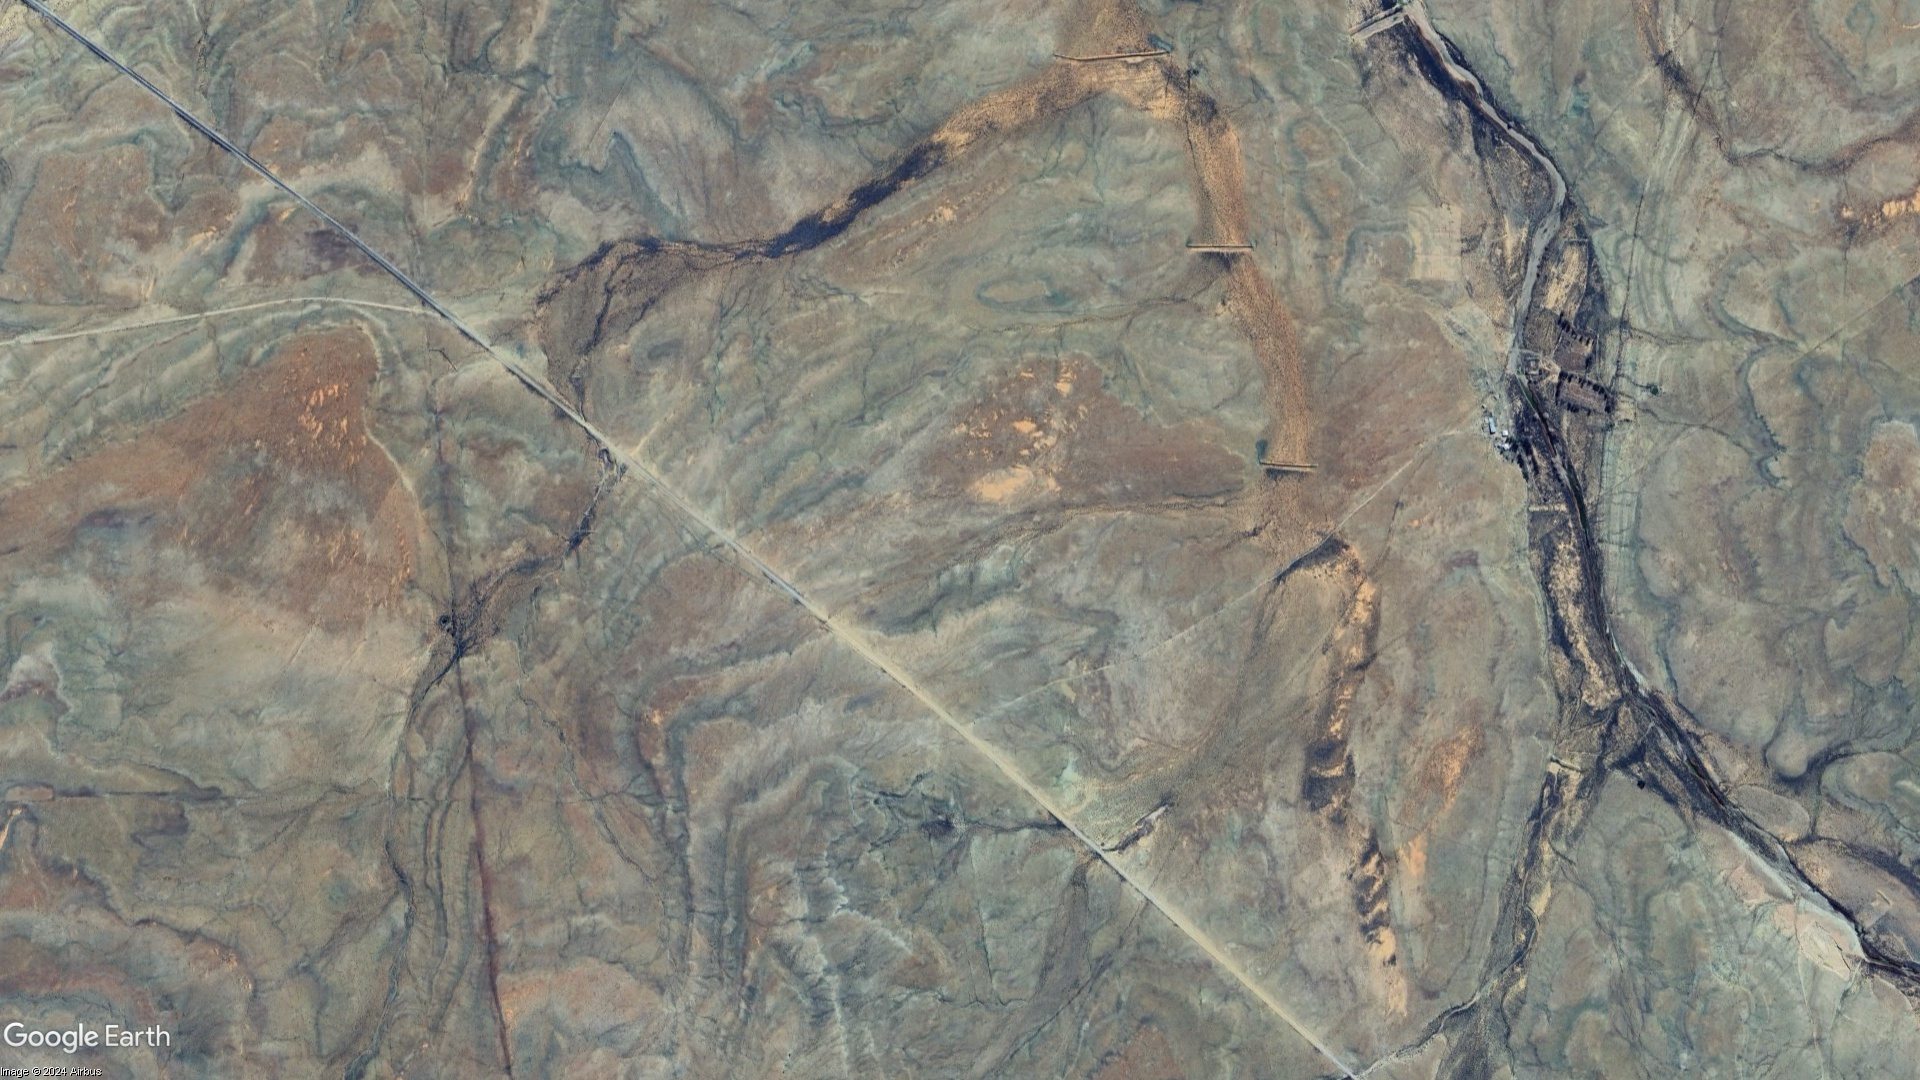
\includegraphics[width=\textwidth]{./Chapter 4/DEMODATASETS/ROCKY.jpg}
        \caption{Example of the ROCKY Dataset.}
        \label{fig:ROCKY}
    \end{minipage}
    
    \vspace{0.15cm} % Add some vertical space between rows
    
    \begin{minipage}{0.4\textwidth}
        \centering
        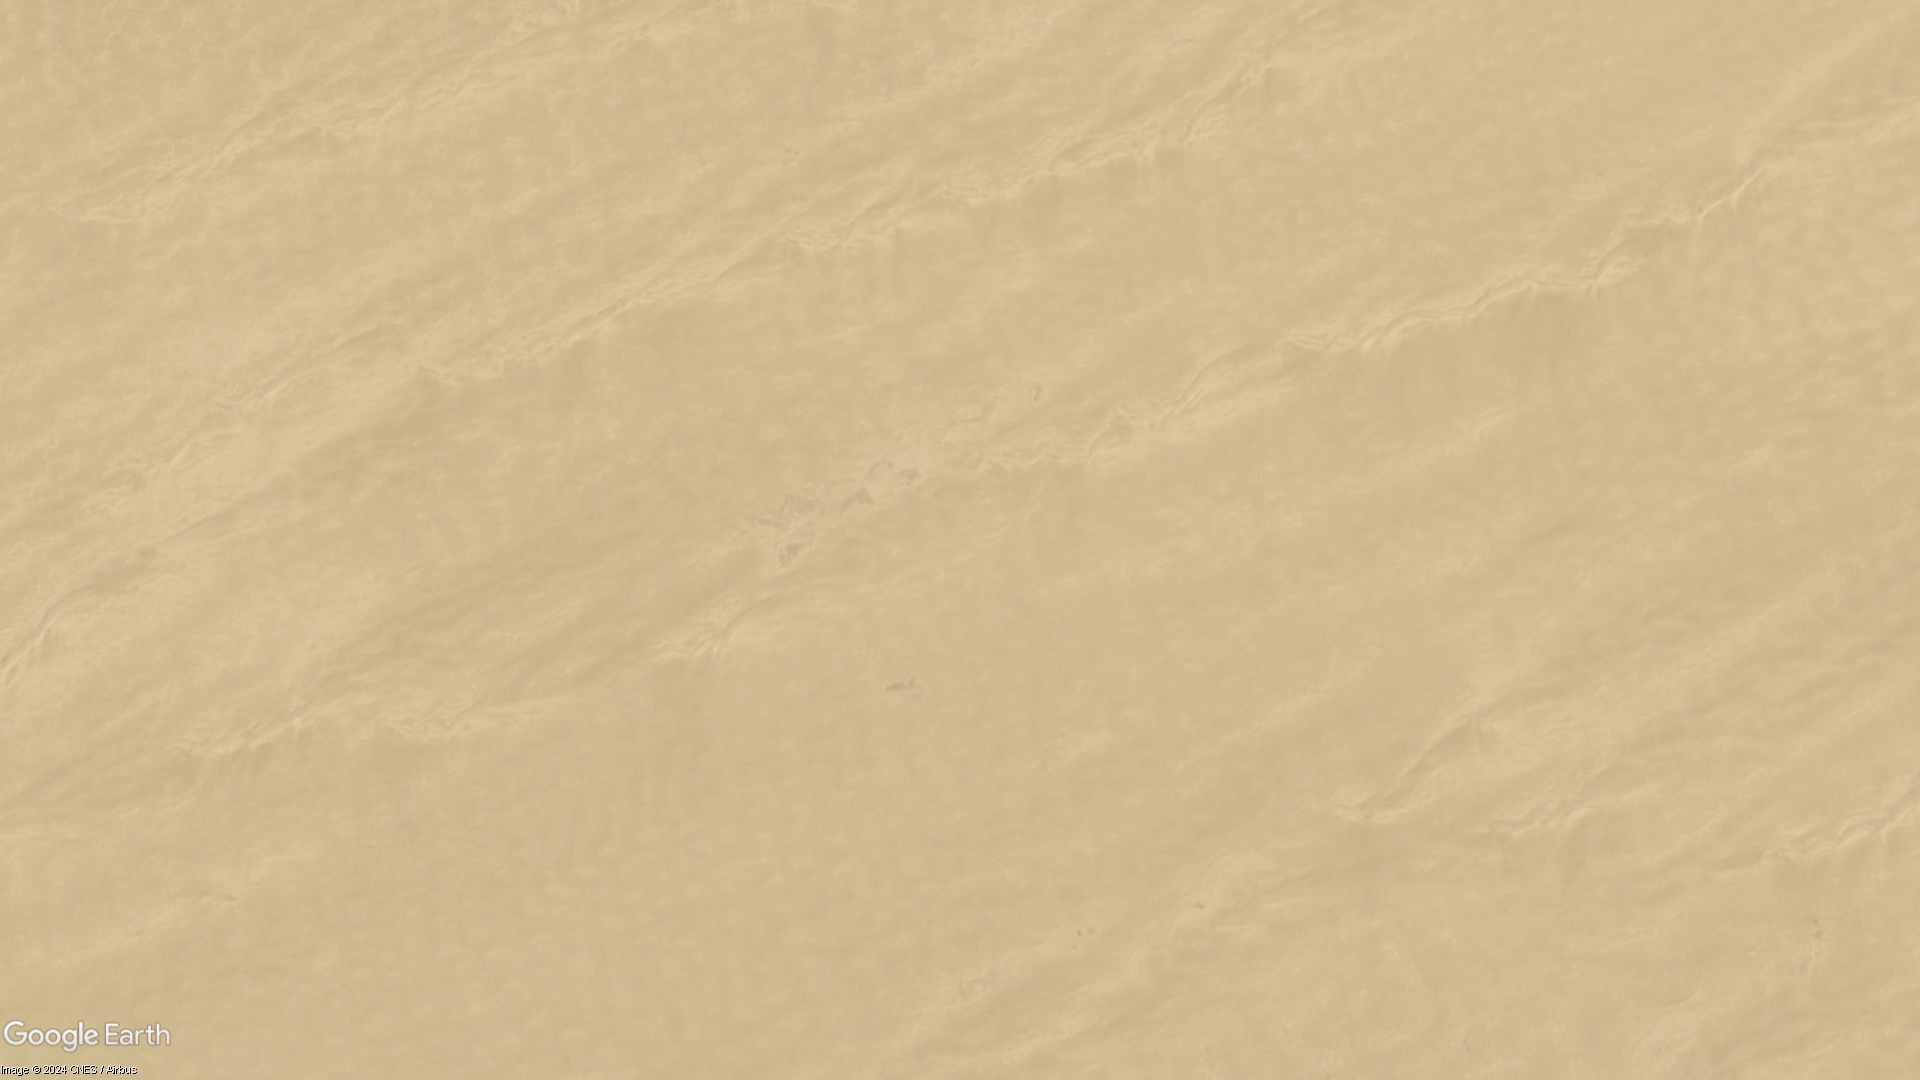
\includegraphics[width=\textwidth]{./Chapter 4/DEMODATASETS/DESERT1.jpg}
        \caption{Example of the DESERT Dataset.}
        \label{fig:DESERT}
    \end{minipage}\hfill
    \begin{minipage}{0.4\textwidth}
        \centering
        
\includegraphics[width=\textwidth]{./Chapter 4/DEMODATASETS/AMAZON.jpg}
        \caption{Example of the AMAZON Dataset.}
        \label{fig:AMAZON}
    \end{minipage}
    
\end{figure}



\subsection{Testing Structure}

Each method is subjected to rigorous testing based on the following criteria:



\textbf{Accuracy}: Evaluated using the radial Root Mean Square Error (RMSE) of Lat-Lon estimations, in meters. This metric provides a clear indication of the method's accuracy in estimating the UAV's position. The accuracy is tested at the end of the pipeline, as errors in prior stages propagate to the final Lat-Lon error. The radial error is given as the mean of the radial errors for all images in the dataset.

\textbf{Runtime}: The runtime of the entire dataset is used for comparison. This includes the time to compute all 15 images for both the with GNSS signal and without GNSS signal phases. Intermediary stages propagate increases in time, and the runtime per line is not necessarily indicative of better performance; hence, the entire runtime is used for comparison. For instance, a method might filter out less keypoints, thereby running faster, but the subsequent stage will take longer due to the increased number of keypoints.

\textbf{Robustness}: This criterion evaluates the method's performance under variation in its parameters, assessing how difficult the method is to tune and how it performs with crudely chosen parameters across datasets. A scoring system from 1-5 is used, where 5 indicates a wide range of parameters offer near-perfect performance, and 1 indicates no static threshold works across datasets. 5 indicates a wide range of parameters offer near optimal performance across datasets; 4 indicates a large range of parameters offer good performance; 3 indicates a small range of parameters offer good performance; 2 indicates a small range of parameters offer usable performance; and 1 indicates that no static threshold works across datasets.


\vspace{-0.5cm}


\section{Feature Detectors}
\vspace{-0.25cm}


This section presents the evaluation results of three feature detectors: ORB, AKAZE (dynamic keypoint targeting implementation), and SuperPoint with LightGlue. Feature detectors were applied to extracting a crude feature layer for rotational estimation, as well as a dense layer for rotational and translational estimation. Initially, all 3 transformations were tested independently for each detector, however, it was seen that the inter-method comparison conclusions were equivalent for each stage. Therefore, to maintain visual brevity, the detectors are applied to all stages and compared once, with the understanding of equivalent comparative independent responses to each stage.

\subsubsection*{Accuracy and Runtime}

Figure ~\ref{fig:rmse_detectors} and Figure ~\ref{fig:runtime_detectors} present the radial error and runtime values for each feature detector across different datasets. AKAZE, utilizing dynamic keypoint targeting, demonstrated the highest accuracy across all datasets while maintaining reasonable runtime. SuperPoint recorded the highest radial errors, particularly in the AMAZON datset, where its training set did not generalize well to the dense, repetitive jungle environment. 

Meanwhile, ORB proved to be the most efficient detector, making it suitable for applications requiring fast processing. SuperPoint demonstrated the longest runtimes across all datasets, highlighting its limited applicability for time-sensitive applications unless optimized with GPU acceleration.

\begin{figure}[H]
    \centering
    \begin{minipage}{0.45\textwidth}
        \centering
        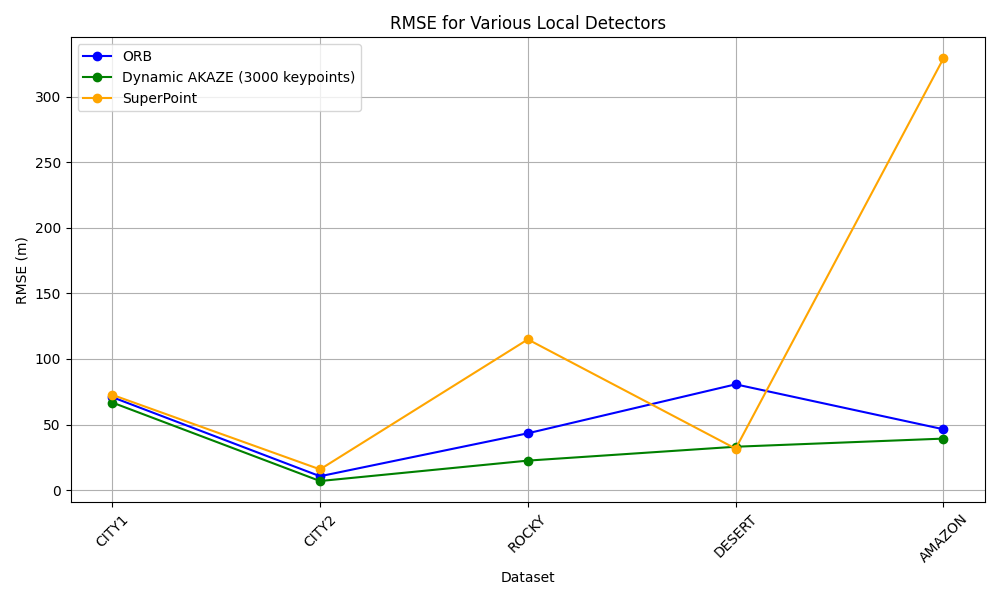
\includegraphics[width=\textwidth]{./Chapter 4/testresults/rmse_detectors.png}
        \caption{Radial Error for Various Feature Detectors.}
        \label{fig:rmse_detectors}
    \end{minipage}\hfill
    \begin{minipage}{0.45\textwidth}
        \centering
        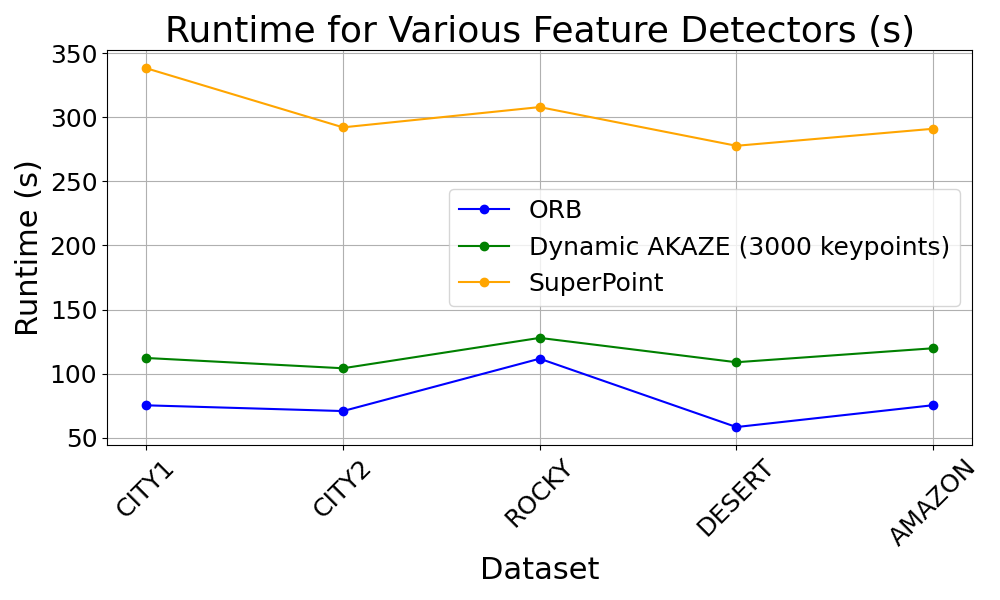
\includegraphics[width=\textwidth]{./Chapter 4/testresults/runtime_detectors.png}
        \caption{Runtime for Various Feature Detectors.}
        \label{fig:runtime_detectors}
    \end{minipage}
\end{figure}


\subsubsection*{Robustness}

All three methods were able to maintain their keypoint targets across environments; however, the quality of those keypoints. SuperPoint consistently achieved equivalent performance across multiple keypoint targets, earning it a robustness score of 5. AKAZE, with its dynamic targeting, was able to generalize well across datasets and only significantly dropped in performance when using below 1000 keypoints, earning a robustness score of 4. ORB, while efficient, required precise tuning to achieve consistently good performance across datasets and was highly sensitive to the target parameter, earning a robustness score of 3.

\subsubsection*{Final Selection of Feature Detectors}

\textbf{Coarse Layer (Initial Detection)}: ORB was chosen for the crude, rotational estimation layer due to its balance of accuracy and efficiency. A range of 3000 - 8000 keypoints maintained reasonable accuracy and runtime, largely due to the invariance of the image similarity estimators to rotational inaccuracies. 3000 keypoints was chosen to prioritize speed and maintain FLANN runtime as per Figure ~\ref{fig:FLANN BF Matcher Keypoint Convergence}.

\textbf{Dense Layer (Refined Detection)}: Dynamic AKAZE was selected for the dense layer due to its consistent performance and robustness and applied to both rotational and translational estimation stages. A range of 3000-5000 keypoints maintained consistent runtime and accuracy. 3000 keypoints was chosen to balance runtime, accuracy, and maintain FLANN performance as per ~\ref{fig:FLANN BF Matcher Keypoint Convergence}.


\vspace{-0.5cm}
\section{Local Feature Matchers}
\vspace{-0.25cm}
This section evaluates two prominent local matchers, BFMatcher and FLANN; LightGLue was implicitly tested in the feature detectors section with SuperPoint. 

\subsubsection*{Accuracy and Runtime Evaluation}

Figure \ref{fig:rmse_flann_bf} presents the radial error in Lat-Lon values for BFMatcher and FLANN across different datasets. The results indicate that while BFMatcher achieves slightly better accuracy in certain cases, FLANN remains highly competitive with only marginally higher RMSE values.

Due to their similar performance, the accuracy was evaluated at varying keypoint targets across datasets to see if their is a specific point of accuracy convergence in the two methods. The difference between accuracy in BFMatcher and FLANN, shown in \ref{fig:FLANN BF Matcher Keypoint Convergence}, indicates that as the number of keypoints increase, the accuracy of both methods converges. Divergence occurs at values below 3000 keypoints, and this should be considered if using FLANN. Notably, FLANN sometimes outperforms BFMatcher (indicated by negative values) due to its approximate matching. For instance, FLANN may find a less similar secondary match for a valid primary match, allowing it to be retained through Lowe's ratio test, where BFMatcher would find a more similar secondary match and discard the valid primary match.

Figure \ref{fig:runtime_flann_bf} shows the runtime comparison for BFMatcher and FLANN across different datasets. FLANN consistently outperforms BFMatcher in terms of speed, with significantly lower execution times across all datasets. Specifically, in the CITY datasets, where the number of keypoints found were significantly higher (no keypoint maximum at this stage), BFMatcher's runtime was significantly higher than FLANN's. This is attributed to FLANN's approximate matching, which scales better with the number of keypoints. 

\begin{figure}[H]
    \centering
    \begin{minipage}{0.45\textwidth}
        \centering
        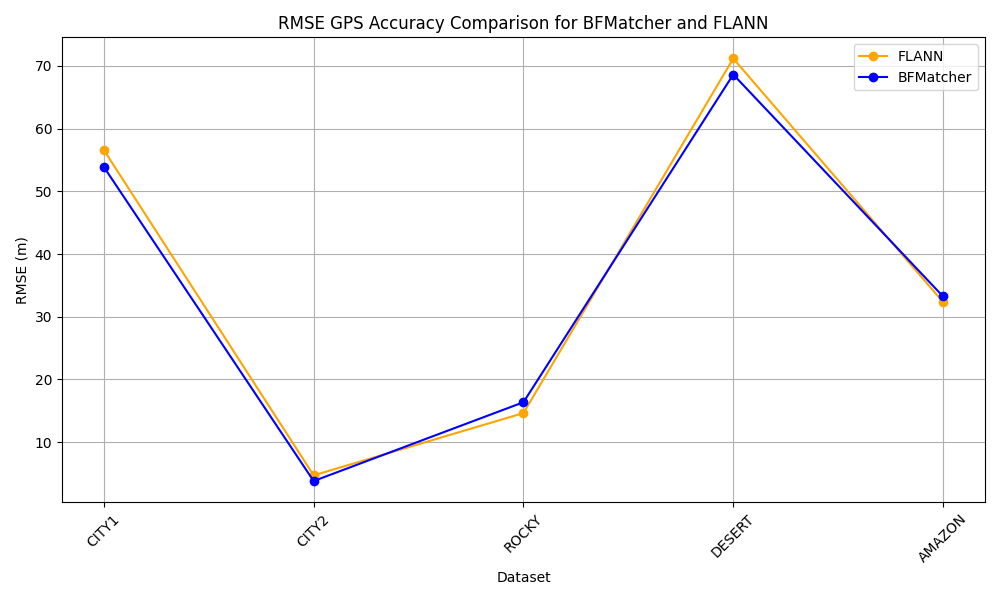
\includegraphics[width=\textwidth]{./Chapter 4/testresults/rmse_flann_bf.png}
        \caption{Radial Error for BFMatcher and FLANN.}
        \label{fig:rmse_flann_bf}
    \end{minipage}\hfill
    \begin{minipage}{0.45\textwidth}
        \centering
        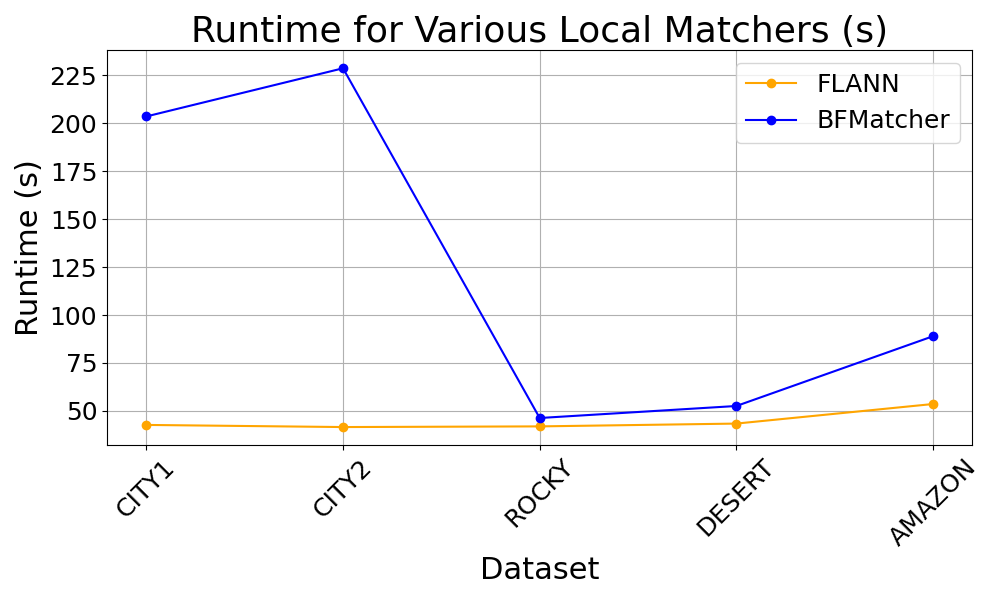
\includegraphics[width=\textwidth]{./Chapter 4/testresults/runtime_flann_bf.png}
        \caption{Runtime Comparison for BFMatcher and FLANN.}
        \label{fig:runtime_flann_bf}
    \end{minipage}
\end{figure}

\begin{figure}[H]
    \centering
    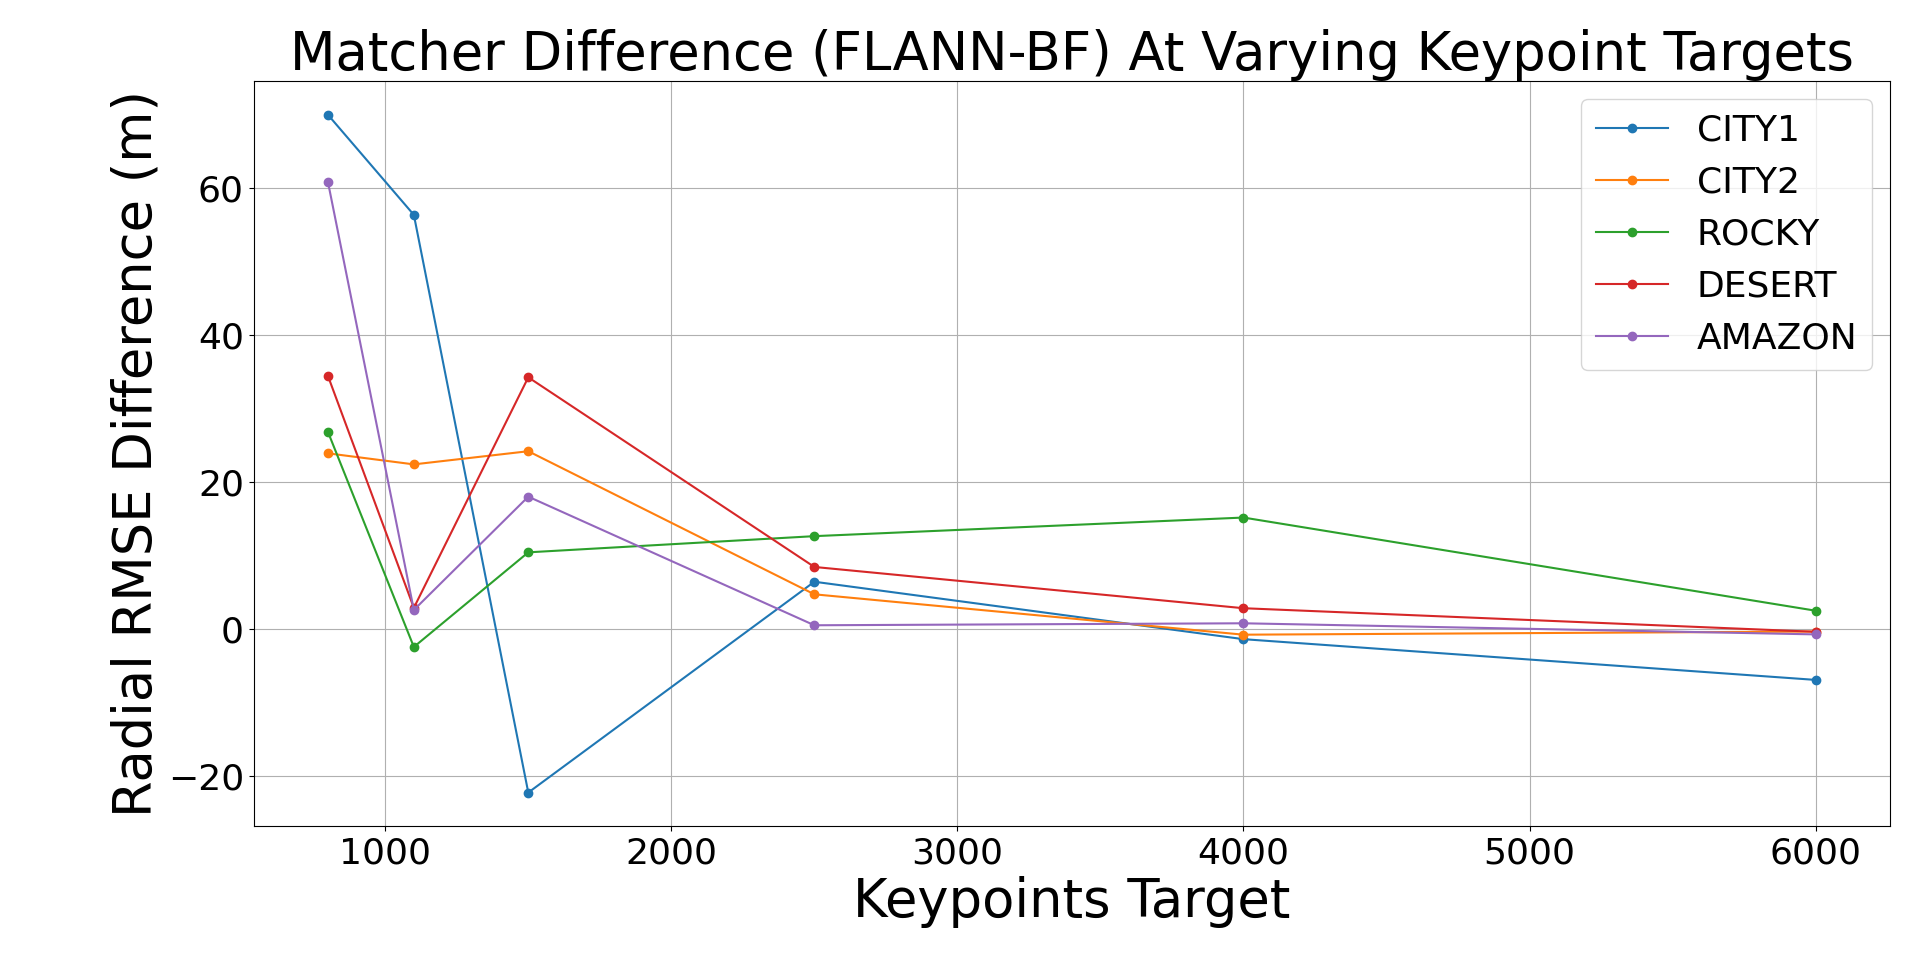
\includegraphics[width=0.45\textwidth]{./Chapter 4/Divergence.png}
    \caption{Convergence in RMSE Lat-Lon Error Between FLANN and BFMatcher Across Keypoint Targets.}
    \label{fig:FLANN BF Matcher Keypoint Convergence} 
\end{figure}

\subsubsection*{Robustness Testing}
BFMatcher did not have any tunable parameters. FLANN had a few parameters that could be tuned, including the number of trees, the number of checks, and the search algorithm. However, FLANN maintained equivalent performance across these ranges; the default parameters were used. 


\subsubsection*{Final Selection of Local Feature Matcher}

Based on the comprehensive evaluation of accuracy, runtime, and robustness, FLANN emerges as the optimal choice for the UAV navigation system. FLANN offers significantly faster runtimes and better scalability while maintaining comparable accuracy to BFMatcher. However, at least 3000 keypoints should be targeted to ensure consistent performance across datasets.

\vspace{-0.5cm}
\section{Planar Transform Estimators}
\vspace{-0.25cm}

This section evaluates the performance of four planar transformation estimation methods: Partial Affine 2D (Rigid Transform plus minor Scaling), Affine 2D, Homography, and Rigid Transform Via SVD. As noted in Section ~\ref{sec:testing_shortlist}, both rotational and translational stages are combined into a single transform evaluation due to conclusion equivalency. For these tests, RANSAC was used on all methods, except the Rigid Transform Via SVD which does not have the method built-in, to filter outliers.

\subsubsection*{Accuracy and Runtime Evaluation}

Figure \ref{fig:rmse_comparison_rotestim} summarizes the RMSE and runtime values across datasets for each rotational estimator method. From the results, it is clear that each method exhibits strengths in different datasets. However, the Rigid SVD method and Partial Affine 2D consistently emerge as the most accurate methods for rotational and translational estimations. The Rigid SVD method slightly outperforms Partial Affine 2D in most datasets, attributed to its strict rigid transformation alignment with dataset characteristics.

The runtime results, shown in \ref{fig:runtime_comparison_rotestim}, are influenced by the degrees of freedom in each method, with more rigid transforms demonstrating the best performance across datasets. SVD proves the fastest due to its lack of iterative optimization.


\begin{figure}[H]
    \centering
    \begin{minipage}{0.45\textwidth}
        \centering
        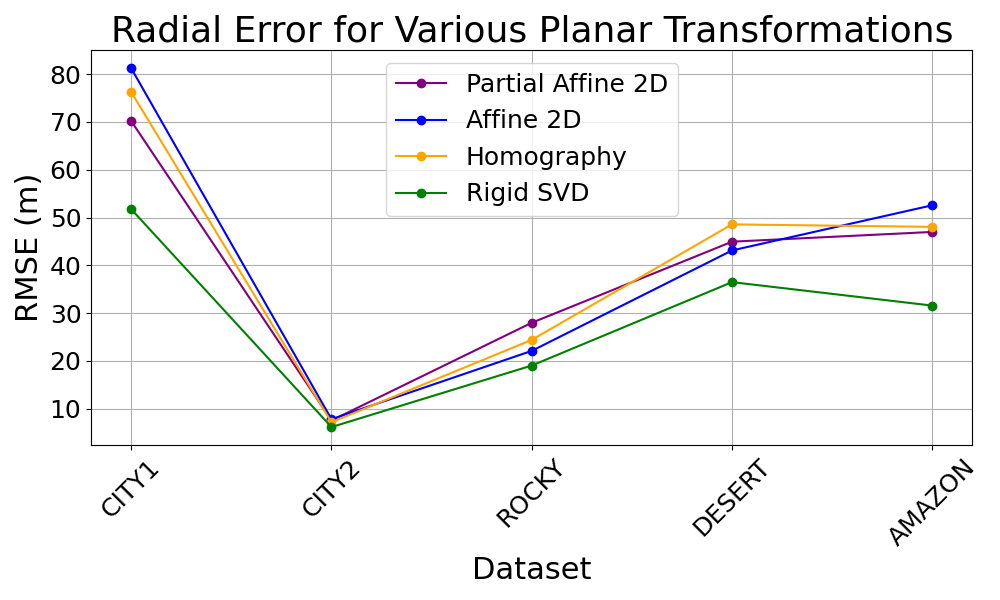
\includegraphics[width=\textwidth]{./Chapter 4/testresults/rmse_planar_estimators.png}
        \caption{RMSE Comparison Across Datasets for Planar Transform Estimators.}
        \label{fig:rmse_comparison_rotestim}
    \end{minipage}\hfill
    \begin{minipage}{0.45\textwidth}
        \centering
        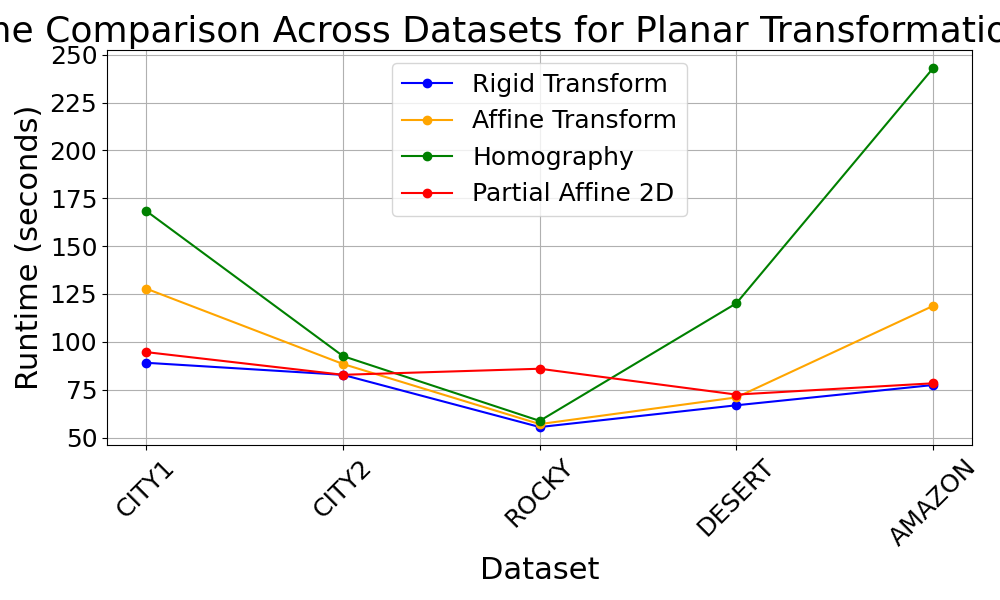
\includegraphics[width=\textwidth]{./Chapter 4/testresults/runtime_planar_estimators.png}
        \caption{Runtime Comparison Across Datasets for Planar Transform Estimators.}
        \label{fig:runtime_comparison_rotestim}
    \end{minipage}
\end{figure}
   
    

\subsubsection*{Robustness Testing}

The openCV methods (partial Affine 2D, Affine 2D, homography) utilize RANSAC, or less often, LMEDS or other outlier rejection methods for robust outlier rejection. These thresholds subtended large differences in accuracy when varied, and required threshold testing from very low to very high thresholds to find the optimal threshold. For more complex, 3-Dimensional, transformations this threshold may be more useful, but it was found to not beat the accuracy of the Rigid SVD method under any threshold in the given application. Thus, OpenCV methods achieve a score of 3 for robustness, while the Rigid SVD method achieves a score of 5 due to its lack of tunable parameters. 

\subsubsection*{Final Selection of Rotational Estimator}

Based on the comprehensive evaluation of accuracy, runtime, and robustness, the rigid transform by SVD emerged as the most suitable estimator for the UAV navigation system. It demonstrated the lowest combined radial RMSE in Lat-Lon across all datasets, and the fastest runtime, largely due to its application-aligned degrees of freedom. Further, it required no parameter tuning, making it highly suitable for real-time UAV applications.




\vspace{-0.5cm}
\section{Image Similarity Estimators}
\vspace{-0.25cm}

Accurate image similarity estimation, or global matching, is essential for UAV navigation systems to choose reasonable images to compare to. They should ensure accuracy and efficiency while maintaining robustness against small rotational offsets. The proximity radius for initial search space reduction was crudely set to 5, but this is not tested as it is a design choice dependent on external factors such as the UAV's speed and the image capture rate. This section specifically evaluates the global matching techniques which are used to estimate the similarity between images to infer the closest match for subsequent heading and position estimation. 


\subsubsection*{Accuracy and Runtime Evaluation}

For clarity, the best match found is implicitly realized in the Lat-Lon estimation error because more similar matches will have a higher number of good matches and subsequently produce lower Lat-Lon estimation errors. 

Figure ~\ref{fig:rmse_global_matching} summarizes the RMSE values (in meters) for the Local Retrofit, Cross Correlation, Histogram, and SSIM methods. The results indicate that the Histogram and Cross-Correlation technique perform near equivalently, with SSIM marginally behind. The Local Retrofit method recorded the highest RMSE values, especially in the DESERT dataset, since its crude detection and matching allowed through many false positives, leading to random choices of the best reference match; it was excluded from further analysis.

Figure ~\ref{fig:runtime_global_matching} compares the computational efficiency of each global matching technique across the five datasets. The Histogram technique demonstrated the most consistent runtimes, followed closely by Cross Correlation. SSIM exhibited the longest runtimes of the remaining methods due to its more complex structural similarity calculations. 


\begin{figure}[H]
    \centering
    \begin{minipage}{0.45\textwidth}
        \centering
        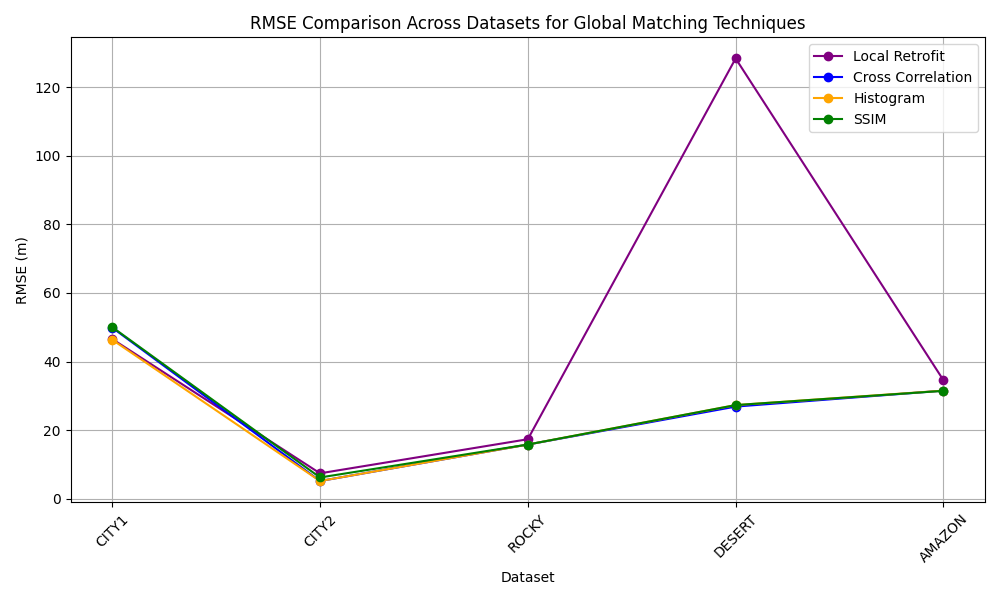
\includegraphics[width=\textwidth]{./Chapter 4/testresults/rmse_global_matching.png}
        \caption{RMSE Comparison Across Datasets for Global Matching Techniques.}
        \label{fig:rmse_global_matching}
    \end{minipage}\hfill
    \begin{minipage}{0.45\textwidth}
        \centering
        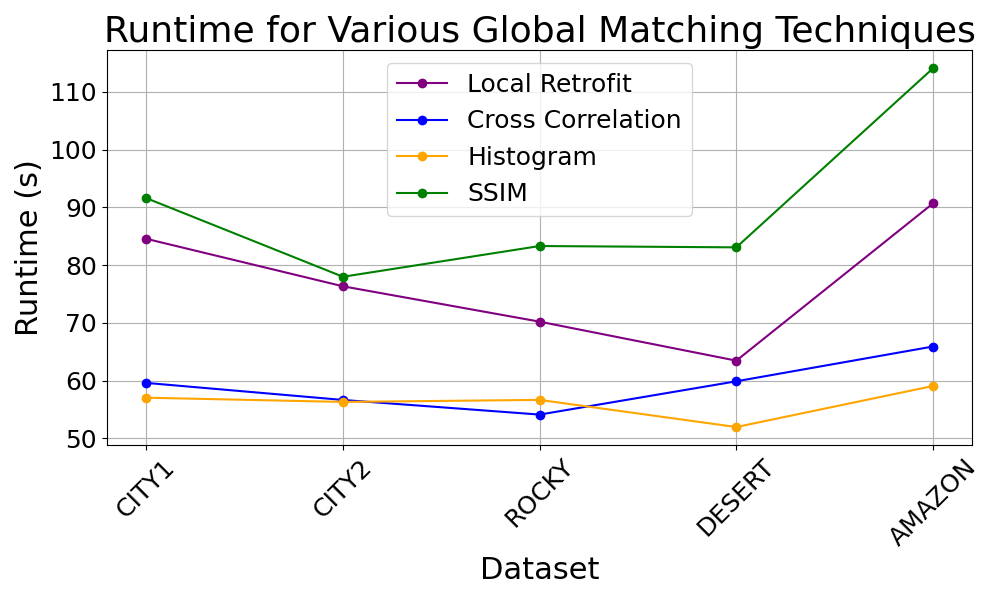
\includegraphics[width=\textwidth]{./Chapter 4/testresults/runtime_global_matching.png}
        \caption{Runtime Comparison Across Datasets for Global Matching Techniques.}
        \label{fig:runtime_global_matching}
    \end{minipage}
\end{figure}

\subsubsection*{Robustness Testing}
The global matching methods did not have any tunable parameters, achieving them a robustness score of 5. However, the local retrofit model had various parameters that could be tuned, including detector type, detector threshold, grid size, match threshold. Further, the runtime and accuracy were extremely difficult to balance, requiring extremely precise tuning to achieve usable performance. As such, the local retrofit model achieved a robustness score of 2. 


\subsubsection*{Considerations for Alignment Prior to Global Matching}

This sections details the considerations when choosing the level of precision of the rotational alignment techniques employed to align the image pairs for unbiased similarity comparisons between the images. This test subjects the estimated internal alignment angle to an additional skew and notes the subsequent response from the global matcher in terms of its chosen best reference match, realized through the location radial error. This was first tested under a 5-degree skew, where no position estimation changes ocurred. Figure ~\ref{fig:percentage_change_comparison_methods} shows the percentage change in Lat-Lon error from the no skew estimate, with a 10-degree skew. Cross-correlation maintains the most similar accuracy, closely followed by histogram and then SSIM. All methods are highly robust to rotational misalignments up to 5 degrees, however, should not exceed this. As such, when employing a rotational alignment technique prior to global matching, a 5-degree skew is tolerable and the choice of detector and matcher may be guided by efficiency rather than accuracy.


\begin{figure}[H]
    \centering
    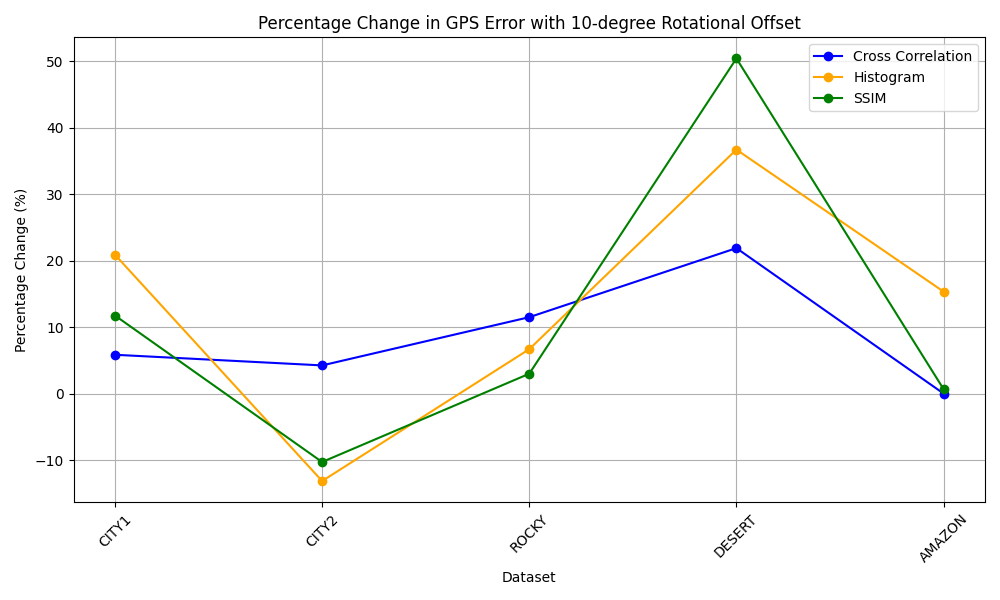
\includegraphics[width=0.5\textwidth]{./Chapter 4/testresults/percentage_change_comparison_methods.png}
    \caption{Percentage Change in Lat-Lon Error with 10-degree Rotational Offset}
    \label{fig:percentage_change_comparison_methods}
\end{figure}





\subsubsection*{Final Selection of Global Matching Technique}

Based on the comprehensive evaluation of accuracy, runtime, and robustness, the Histogram technique is identified and chosen as the most suitable global matching method for the system. Histogram consistently provided superior performance in terms of both RMSE and runtime, whilst maintaining sufficient robustness to rotational error. 



\vspace{-0.5cm}
\section{Optimization Techniques}
\vspace{-0.25cm}

Several methods were used to enhance the performance of the UAV navigation system, focusing on filtering image matches to balance noise and maintain stability within the point sets. These optimization techniques are simpler to implement, and not assessed with the same depth as those in previous sections. Since precise parameter optimization was not the primary goal of this pipeline, parameters were tuned approximately, with functional ranges documented.




\subsubsection*{Planar Transform Outlier Rejection Methods}

Two outlier rejection methods, LMEDS (Least Median of Squares) and RANSAC (Random Sample Consensus), were evaluated for match filtration. Both methods performed near equivalently, with LMEDS displaying a slightly lower radial error. LMEDS was also significantly faster than RANSAC, making it the preferred choice for planar transform outlier rejection. The results are summarized in Figure \ref{fig:rmse_comparisonlmeds} and Figure \ref{fig:runtime_comparisonlmeds}. Both thresholds require precise tuning, with LMEDS requiring slightly less tuning. Both methods achieved a robustness score of 3, as they required precise tuning to achieve optimal performance across datasets. However, these techniques were not used in the prior optimal pipeline, hence their exclusion from the final selection.

\begin{figure}[H]
    \centering
    \begin{minipage}{0.45\textwidth}
        \centering
        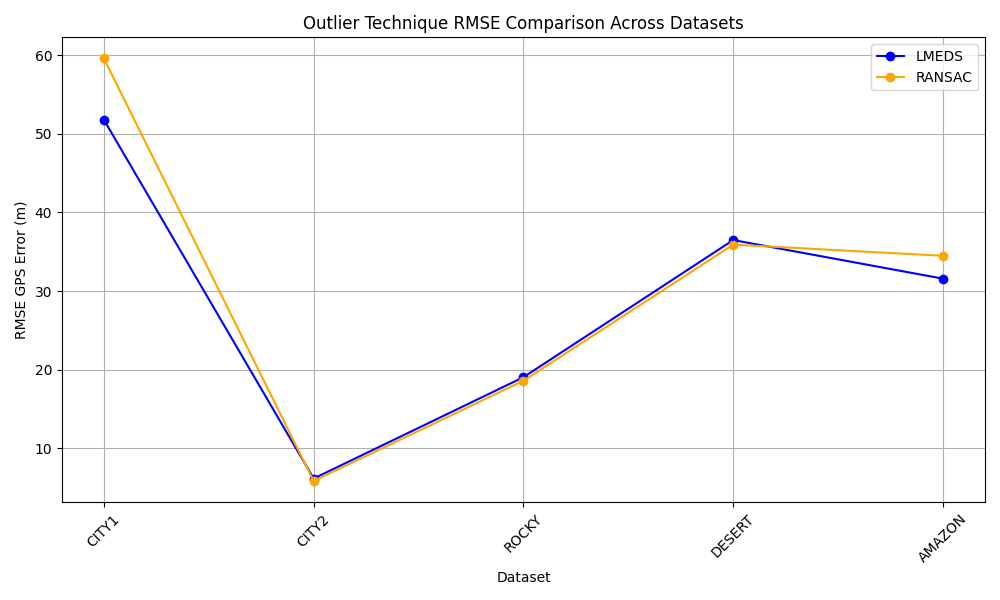
\includegraphics[width=\textwidth]{./Chapter 4/testresults/ransaclmedsrmse.png}
        \caption{Radial Lat-Lon RMSE Comparison Across Datasets for LMEDS and RANSAC.}
        \label{fig:rmse_comparisonlmeds}
    \end{minipage}\hfill
    \begin{minipage}{0.45\textwidth}
        \centering
        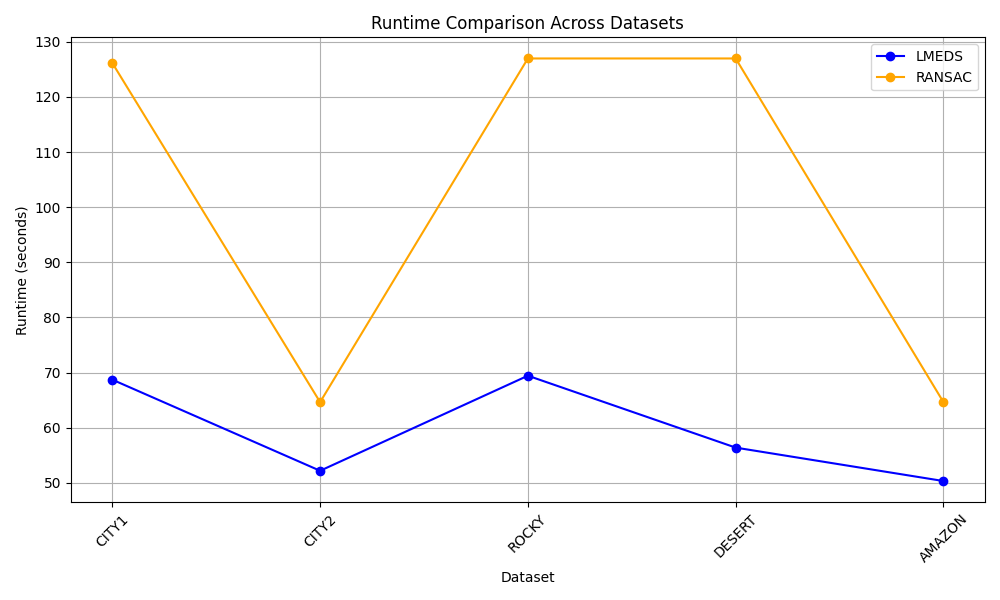
\includegraphics[width=\textwidth]{./Chapter 4/testresults/ransaclmedsruntime.png}
        \caption{Runtime Comparison Across Datasets for LMEDS and RANSAC.}
        \label{fig:runtime_comparisonlmeds}
    \end{minipage}
\end{figure}




\subsubsection*{Lowe's Ratio Test}

Lowe's Ratio Test was utilized to filter keypoint matches by comparing the distance of the best match to that of the second-best match. Initially, a static threshold was applied to determine match quality. However, this static approach was insufficient for handling the variability across diverse datasets, resulting in inconsistent accuracy. To improve robustness, a dynamic thresholding strategy was adopted. This approach involves setting an initial threshold and incrementally increasing it, thereby allowing greater leniency until a predefined number of matches or percentage of the keypoints is found.

A lower initial threshold and lower increment value increased the likelihood of approaching the desired match count but impacted runtime. The initial threshold was set to 0.7, and the increment was established at 0.05. This balanced efficiency and accuracy. Working ranges are between 0.5-0.75 and 0.025-0.1, respectively. 

Through testing, a target of 500 keypoints was selected for its ability to consistently maintain stability across diverse datasets. The working range for reliable performance was found to be 300 to 700 keypoints. Additionally, to prevent low-quality matches from entering the system when fewer keypoints were detected, a maximum match-to-keypoint ratio of 75\% was implemented to ensure enough keypoints were found. 
 


\subsubsection*{N-Match or Absolute Thresholding}

Absolute Thresholding, or N-Match Thresholding, involves filtering keypoint matches based on a fixed number of matches or a specific descriptor distance threshold. The latter proved to be more effective in generalizing across datasets, and was subsequently chosen. 

The method was applied prior to Lowe's filtering, with a lenient threshold, to ensure it aids in computation for subsequent stages while not removing potential matches. This step was especially beneficial in removing excessive keypoints in instances when the detector found abnormally high numbers of keypoints in specific images. 

During the testing phase, various match threshold values between 700 and 2500 keypoints were found to perform relatively equivalently. Thresholds well below this limit were found to be too restrictive, while those above the limit had negligible effect. A threshold of 1000 keypoints was chosen due to significant gains in runtime relative to the upper limit, with negligible effect on accuracy. 


\vspace{-0.5cm}
\section{Summary}
\vspace{-0.25cm}
The following methods were selected based on the comprehensive evaluation of accuracy, runtime, and robustness across diverse datasets:


The feature detector chosen was \textbf{ORB} (3000) for the coarse detection layer, and \textbf{AKAZE} (3000) for the dense layer. The local matcher chosen was \textbf{FLANN}. The planar transformation estimator chosen was \textbf{Rigid Transform Via SVD}. The image similarity estimator chosen was \textbf{Histogram}. The optimization techniques chosen were \textbf{N-Match Thresholding} (1000), and \textbf{Lowe's Filtering} (500). 

These methods are employed in the results section. 